% ============================================================
%  BÁO CÁO ĐỒ ÁN MÔN HỌC SS004.R11 – GAME TETRIS – TUẦN 1
%  Biên dịch bằng XeLaTeX (Overleaf: Menu -> Compiler -> XeLaTeX)
%  Chỗ cần điền: tìm "[" màu đỏ, hoặc chỉnh các \newcommand ở khối THÔNG TIN NHÓM
% ============================================================
\documentclass[a4paper]{article}
\usepackage[fontsize=13pt]{scrextend} % Cỡ chữ nội dung chuẩn 13pt

% --- Font chữ (Biên dịch bằng XeLaTeX) ---
\usepackage{fontspec}
\setmainfont{Times New Roman}
\setmonofont{DejaVu Sans Mono}[Scale=0.85]

% --- Căn lề chuẩn khóa luận/tiểu luận ---
\usepackage[a4paper, left=3cm, right=2cm, top=2.5cm, bottom=2.5cm]{geometry}

% --- Các gói hỗ trợ ---
\usepackage[table]{xcolor}
\usepackage{graphicx}
\usepackage{booktabs, tabularx, array, multirow}
\usepackage{enumitem}
\usepackage{etoolbox}
\usepackage{float}
\usepackage{amsmath}
\usepackage{tikz}
\usetikzlibrary{arrows.meta}

% --- Giãn dòng & Đoạn văn ---
\usepackage{setspace}
\setstretch{1.3} % Chuẩn 1.5 lines của Word (đổi lại 1.5 nếu muốn thưa hơn)
\usepackage{indentfirst}
\setlength{\parindent}{1.27cm}
\setlength{\parskip}{0pt}
\widowpenalty=10000
\clubpenalty=10000
\setlist{itemsep=2pt, topsep=3pt, parsep=0pt}

% --- Tự động cỡ chữ 11pt cho toàn bộ bảng tabularx ---
\renewcommand{\arraystretch}{1.25}
\AtBeginEnvironment{tabularx}{\linespread{1.1}\fontsize{11pt}{13.2pt}\selectfont}

% --- Header & Footer ---
\usepackage{fancyhdr}
\pagestyle{fancy}
\fancyhf{}
\renewcommand{\headrulewidth}{0pt}
\renewcommand{\footrulewidth}{0pt}
\fancyfoot[C]{\thepage}

% --- Việt hóa & Định dạng Chú thích (Caption) ---
\usepackage{caption}
\counterwithin{table}{section}
\counterwithin{figure}{section}
\renewcommand{\contentsname}{Mục lục}
\renewcommand{\tablename}{Bảng}
\renewcommand{\figurename}{Hình}
\renewcommand{\refname}{Tài liệu tham khảo}

\captionsetup{
  font={normalsize,bf}, % Cỡ 13pt, in đậm toàn bộ
  labelfont=bf,
  justification=centering,
  singlelinecheck=false,
  labelsep=colon
}
\captionsetup[table]{skip=6pt, labelsep=period}
\captionsetup[figure]{position=bottom, skip=6pt}
\newcommand{\nguon}[1]{\par\vspace{3pt}\noindent\hfill\textit{\small Nguồn: #1}}

% --- Màu sắc ---
\definecolor{uitblue}{HTML}{1F4E79}
\definecolor{headfill}{HTML}{DCE6F1}
\definecolor{todored}{HTML}{C00000}

% --- Định dạng Tiêu đề các cấp ---
\usepackage{titlesec}
\setcounter{secnumdepth}{4}
\setcounter{tocdepth}{3}

% Cấp 1 - Chương: 14pt, đậm, IN HOA (đổi \raggedright thành \centering nếu muốn căn giữa)
\titleformat{\section}[block]
  {\raggedright\fontsize{14pt}{21pt}\selectfont\bfseries\color{black}}
  {CHƯƠNG \thesection.\ }{0pt}{\MakeUppercase}
\titlespacing{\section}{0pt}{6pt}{12pt}

\titleformat{name=\section, numberless}[block]
  {\centering\fontsize{14pt}{21pt}\selectfont\bfseries\color{black}}
  {}{0pt}{\MakeUppercase}

% Cấp 2 - Tiểu mục 1.1: 13pt, đậm, căn trái
\titleformat{\subsection}[block]
  {\raggedright\fontsize{13pt}{19.5pt}\selectfont\bfseries\color{black}}
  {\thesubsection.\ }{0pt}{}
\titlespacing{\subsection}{0pt}{6pt}{0pt}

% Cấp 3 - Tiểu mục 1.1.1: 13pt, đậm + nghiêng, căn trái
\titleformat{\subsubsection}[block]
  {\raggedright\fontsize{13pt}{19.5pt}\selectfont\bfseries\itshape\color{black}}
  {\thesubsubsection.\ }{0pt}{}
\titlespacing{\subsubsection}{0pt}{0pt}{0pt}

% Cấp 4 - Tiểu mục 1.1.1.1: 13pt, chữ thường, căn trái
\titleformat{\paragraph}[block]
  {\raggedright\fontsize{13pt}{19.5pt}\selectfont\normalfont}
  {\theparagraph.\ }{0pt}{}
\titlespacing{\paragraph}{0pt}{0pt}{0pt}

% --- Mục lục ---
\usepackage[titles]{tocloft}
\renewcommand{\cftsecpresnum}{CHƯƠNG }
\renewcommand{\cftsecaftersnum}{.}
\cftsetindents{section}{0em}{6.2em}
\renewcommand{\cftsecfont}{\bfseries}
\renewcommand{\cftsecleader}{\cftdotfill{\cftdotsep}}
\renewcommand{\cftsubsecaftersnum}{.}
\cftsetindents{subsection}{1.5em}{2.6em}

% --- Macro tiện ích ---
\newcommand{\todo}[1]{\textcolor{todored}{[#1]}}
\newcommand{\hl}[1]{\cellcolor{headfill}\textbf{#1}}
\newcommand{\chuky}[1]{\IfFileExists{#1}{\includegraphics[height=1.1cm]{#1}}{\rule{0pt}{1.1cm}}}
\newcommand{\minhchung}[3]{%
  \IfFileExists{#1}{\begin{figure}[H]\centering
  \includegraphics[width=#2\linewidth]{#1}\caption{#3}\end{figure}}{}}

% --- Liên kết (nên nạp cuối cùng trong preamble) ---
\usepackage[colorlinks=true, linkcolor=black, urlcolor=blue!60!black]{hyperref}
% ============================================================
%  THÔNG TIN NHÓM – CHỈ CẦN SỬA Ở ĐÂY
% ============================================================
\newcommand{\tennhom}{{Nhom08}}
\newcommand{\gvien}{{ThS. Nguyễn Văn Toàn}}
\newcommand{\ngaylap}{{11/11/2026}}

% 5 thành viên – KHÔNG có trưởng nhóm, thứ tự chỉ để đánh số
\newcommand{\tvA}{{Lưu Chí Bảo}} \newcommand{\mssvA}{{25520137}} \newcommand{\mailA}{{25520137}@gm.uit.edu.vn}
\newcommand{\tvB}{{Nguyễn Thành Đạt}} \newcommand{\mssvB}{{25520288}} \newcommand{\mailB}{{25520288}@gm.uit.edu.vn}
\newcommand{\tvC}{{Nguyễn Thế Minh}} \newcommand{\mssvC}{{25521124}} \newcommand{\mailC}{{25521124}@gm.uit.edu.vn}
\newcommand{\tvD}{{Trương Công Lĩnh}} \newcommand{\mssvD}{{25521011}} \newcommand{\mailD}{{25521011}@gm.uit.edu.vn}
\newcommand{\tvE}{{Đinh Mạc Khải Nam}} \newcommand{\mssvE}{{25521152}} \newcommand{\mailE}{{25521152}@gm.uit.edu.vn}

% ============================================================
%  MÀU & HÌNH TETRIS (vẽ bằng TikZ)
% ============================================================
\definecolor{tI}{HTML}{00BCD4} \definecolor{tO}{HTML}{FFC107}
\definecolor{tT}{HTML}{9C27B0} \definecolor{tS}{HTML}{4CAF50}
\definecolor{tZ}{HTML}{F44336} \definecolor{tJ}{HTML}{2962FF}
\definecolor{tL}{HTML}{FF9800}

% \tetro{x/y,x/y,...}{màu}{cỡ ô}
\newcommand{\tetro}[3]{\foreach \x/\y in {#1}{%
  \fill[#2,draw=black!55,line width=0.3pt] (\x*#3,\y*#3) rectangle ++(#3,#3);}}

\begin{document}

% ============================================================
%  TRANG BÌA
% ============================================================
\begin{titlepage}
\centering
\begin{tikzpicture}[remember picture,overlay]
  \draw[line width=2.6pt] ([shift={(1.3cm,1.3cm)}]current page.south west)
        rectangle ([shift={(-1.3cm,-1.3cm)}]current page.north east);
  \draw[line width=0.7pt] ([shift={(1.5cm,1.5cm)}]current page.south west)
        rectangle ([shift={(-1.5cm,-1.5cm)}]current page.north east);
\end{tikzpicture}
\centering
\vspace*{0.3cm}
{\large\bfseries ĐẠI HỌC QUỐC GIA TP. HỒ CHÍ MINH}\\[4pt]
{\large\bfseries TRƯỜNG ĐẠI HỌC CÔNG NGHỆ THÔNG TIN}\\[1.2cm]

% Logo: upload file logo-uit.png lên Overleaf
\IfFileExists{logo-uit.png}{
\includegraphics[width=4.6cm]{logo-uit.png}}%
  {\fbox{\parbox[c][3.4cm][c]{4.2cm}{\centering\todo{Chèn logo UIT\\(logo-uit.png)}}}}\\[1.4cm]

{\Large\bfseries BÁO CÁO ĐỒ ÁN MÔN HỌC}\\[0.5cm]
{\large Môn học: SS004 – Lớp: R11}\\[0.9cm]
{\fontsize{26}{30}\selectfont\bfseries\color{uitblue} GAME TETRIS}\\[0.4cm]
{\large\itshape Xây dựng game Tetris bằng C++ (chạy trên console)}\\[0.9cm]
{\large\bfseries BÁO CÁO TUẦN 1}\\[3pt]
{\normalsize Hợp đồng nhóm – Các link công cụ – Giới thiệu và hướng dẫn chơi game}\\[1.1cm]

\begin{flushleft}
\linespread{1.3}\selectfont
\renewcommand{\arraystretch}{1}
\hspace{1.3cm}\begin{tabular}{@{}l l l@{}}
\textbf{Nhóm:}               & \multicolumn{2}{l}{\tennhom}\\[8pt]
\textbf{Giảng viên:}         & \multicolumn{2}{l}{\gvien}\\[8pt]
\textbf{Sinh viên thực hiện:}& \tvA & -- \mssvA\\
                             & \tvB & -- \mssvB\\
                             & \tvC & -- \mssvC\\
                             & \tvD & -- \mssvD\\
                             & \tvE & -- \mssvE\\[8pt]
\textbf{Tuần:}               & \multicolumn{2}{l}{1 (09/11/2026 -- 15/11/2026)}\\
\end{tabular}
\end{flushleft}
\vfill
{\bfseries TP. HỒ CHÍ MINH, THÁNG 11 NĂM 2026}
\thispagestyle{empty}
\end{titlepage}
\clearpage
\pagenumbering{gobble}
\renewcommand{\contentsname}{MỤC LỤC}

\tableofcontents

\clearpage
\pagenumbering{arabic}
\setcounter{page}{1}
\newpage

% ============================================================
%  PHẦN 1 – HỢP ĐỒNG NHÓM
% ============================================================
\section{HỢP ĐỒNG NHÓM}
\subsection{Thông tin chung}
\begin{table}[H]
\centering
\begin{tabularx}{\linewidth}{|p{4.3cm}|X|}
\hline
\textbf{Tên môn học} & Kỹ năng nghề nghiệp (SS004.R11) \\ \hline
\textbf{Giảng viên hướng dẫn} & ThS. Nguyễn Văn Toàn \\ \hline
\textbf{Tên nhóm} & Nhom08 \\ \hline
\textbf{Đề tài đồ án} & Xây dựng game Tetris bằng C++ (chạy trên console) \\ \hline
\textbf{Ngày lập hợp đồng} & 11/11/2026 \\ \hline
\textbf{Hạn nộp tuần 1} & 22:00, ngày 12/11/2026 \\ \hline
\end{tabularx}
\vspace{8pt}
\caption{Thông tin chung của hợp đồng nhóm}
\label{tab:thongtin}
\end{table}

\subsection{Thành viên nhóm}
\begin{table}[H]
\centering
\begin{tabularx}{\linewidth}{|>{\centering\arraybackslash}p{1.2cm}|X|>{\centering\arraybackslash}p{2.8cm}|X|}
\hline
\textbf{STT} & \multicolumn{1}{c|}{\textbf{Họ và tên}} & \textbf{MSSV} & \multicolumn{1}{c|}{\textbf{Email}} \\ \hline
1 & Lưu Chí Bảo & 25520137 & \texttt{25520137@gm.uit.edu.vn} \\ \hline
2 & Nguyễn Thành Đạt & 25520288 & \texttt{25520288@gm.uit.edu.vn} \\ \hline
3 & Nguyễn Thế Minh & 25521124 & \texttt{25521124@gm.uit.edu.vn} \\ \hline
4 & Trương Công Lĩnh & 25521011 & \texttt{25521011@gm.uit.edu.vn} \\ \hline
5 & Đinh Mạc Khải Nam & 25521152 & \texttt{25521152@gm.uit.edu.vn} \\ \hline
\end{tabularx}
\vspace{8pt}
\caption{Danh sách thành viên}
\label{tab:thanhvien}
\end{table}

\subsection{Mục tiêu và nguyên tắc chung}
\textbf{Mục tiêu.} Cả nhóm cam kết hoàn thành game Tetris đúng yêu cầu của môn học và đúng hạn. Nhóm bám sát khung mã và video hướng dẫn của giảng viên (mảng \texttt{board}, mảng \texttt{blocks} 4$\times$4, các hàm \texttt{canMove}, \texttt{block2Board}, \texttt{boardDelBlock}, \texttt{removeLine}\ldots) rồi mới mở rộng thêm chức năng ở Mục~\ref{sec:chucnang}. Mỗi thành viên đều viết mã thật và hiểu rõ phần mình làm.

\textbf{Nguyên tắc bình đẳng.}
\begin{itemize}

  \item Khối lượng công việc chia đều: mỗi người một mô-đun cốt lõi, một chức năng mở rộng, một phần báo cáo và một lượt review chéo (Bảng~\ref{tab:phancong}).
  \item Các việc ``đầu mối'' như ghi biên bản họp, nộp bài trên website môn học được \emph{luân phiên} theo Bảng~\ref{tab:luanphien}; người đảm nhận chỉ thực hiện thao tác, không có thêm quyền quyết định.
\end{itemize}

\subsection{Phân công công việc}
Cách chia dựa trên các thành phần của game mà giảng viên liệt kê trong video (bảng chơi, khối gạch, di chuyển, rơi tự động, va chạm, xóa dòng, sinh khối mới, game over, hiển thị console).

\begin{table}[H]
\centering
\renewcommand{\tabularxcolumn}[1]{m{#1}}
\begin{tabularx}{\linewidth}{|c|>{\hsize=1.3\hsize\raggedright\arraybackslash}X|>{\hsize=0.85\hsize\raggedright\arraybackslash}X|>{\hsize=0.85\hsize\raggedright\arraybackslash}X|c|}
\hline
\textbf{TV} &
\centering\arraybackslash\textbf{Mô-đun cốt lõi (khung của thầy)} &
\centering\arraybackslash\textbf{Chức năng mở rộng} &
\centering\arraybackslash\textbf{Phần báo cáo} &
\textbf{Thành viên} \\ \hline
1 & Bảng chơi \& hiển thị: \texttt{board}, \texttt{initBoard}, \texttt{draw} & Giao diện: màu theo loại khối, khung thông tin & Mục~3.1: Giới thiệu chung về trò chơi Tetris & Bảo \\ \hline
2 & Khối gạch: mảng \texttt{blocks}, sinh khối ngẫu nhiên & Đủ 7 loại khối, mỗi loại một khối & Mục~1: Hợp đồng nhóm & Đạt \\ \hline
3 & Di chuyển \& va chạm: \texttt{canMove}, phím \texttt{a}/\texttt{d}/\texttt{x} & Xoay khối 90$^\circ$ và phím xoay & Mục~3.3: Các chức năng chính & Minh \\ \hline
4 & Đặt/xóa khối và cố định khối: \texttt{block2Board}, \texttt{boardDelBlock}, rơi tự động & Điểm số, level, tốc độ rơi tăng dần & Mục~3.2: Cách chơi & Lĩnh \\ \hline
5 & Xóa dòng đầy: \texttt{removeLine} & Menu, tạm dừng, game over, chơi lại & Mục~2: link công cụ; hình minh họa & Nam \\ \hline
\end{tabularx}
\vspace{8pt}
\caption{Phân công công việc (mỗi người đều có 4 phần việc tương đương)}
\label{tab:phancong}
\end{table}
\begin{table}[H]
\centering

\begin{tabularx}{\linewidth}{|p{4.8cm}|X|}
\hline
\multicolumn{1}{|c|}{\textbf{Việc điều phối}} & \multicolumn{1}{c|}{\textbf{Cách luân phiên}} \\ \hline
Người nộp link Overleaf & Nguyễn Thành Đạt; hai người khác xác nhận đã nộp thành công \\ \hline
Người ghi biên bản họp & Lần lượt Đạt $\to$ Nam $\to$ Bảo $\to$ Lĩnh $\to$ Minh \\ \hline
Người ghép và rà lỗi cuối báo cáo & Mỗi người tự cập nhật mục của mình trên Overleaf, người khác góp ý nếu có sai sót \\ \hline
Người duyệt Pull Request & Các thành viên trong nhóm \\ \hline
\end{tabularx}
\vspace{8pt}
\caption{Các việc điều phối được luân phiên}
\label{tab:luanphien}
\end{table}


\subsection{Giao tiếp và họp nhóm}
\begin{itemize}
  \item Họp nhóm tối thiểu một lần mỗi tuần (trực tuyến); nội dung họp và việc cần làm được ghi lên Trello.
  \item Trao đổi hằng ngày qua Slack; tin nhắn liên quan đến phần việc của mình phải được trả lời trong vòng 24 giờ.
  \item Mỗi công việc là một thẻ Trello, ghi rõ người phụ trách, người review và hạn hoàn thành.
  \item Hạn nội bộ sớm hơn hạn nộp ít nhất 24 giờ (trước 22:00 ngày 11/11/2026) để còn thời gian ghép và kiểm tra.
  \item Góp ý nhắm vào nội dung công việc, không công kích cá nhân; mọi ý kiến đều được lắng nghe.
\end{itemize}

\subsection{Quy tắc ra quyết định}
\begin{itemize}
  \item Quyết định thông thường (nội dung, cách trình bày, thứ tự việc, đổi người làm một đầu việc): cần ít nhất \textbf{3/5} thành viên đồng ý.
  \item Quyết định quan trọng (sửa hợp đồng, đổi đề tài hoặc cách chia mô-đun, điều chỉnh tỉ lệ đóng góp): cần ít nhất \textbf{4/5} thành viên đồng ý.
  \item Biểu quyết trong một thread riêng trên Slack, thời hạn 24 giờ; thành viên không phản hồi trong thời hạn không được tính là đồng ý.
  \item Thành viên thuộc ý kiến thiểu số được ghi ý kiến vào biên bản; sau khi quyết định được thông qua, cả nhóm cùng thực hiện.
\end{itemize}

\subsection{Quy tắc sử dụng Git}
\begin{itemize}
  \item Không đẩy trực tiếp lên nhánh \texttt{main}; mỗi người làm trên nhánh riêng và gộp qua Pull Request, do người khác review.
  \item Commit nhỏ, mỗi commit một việc, thông điệp rõ nghĩa (ví dụ: \texttt{Add T block}).
  \item Mục tiêu tối thiểu của nhóm: 50 commit, 5--6 nhánh, và ít nhất 3 lần tự giải quyết xung đột (conflict) khi gộp mã.
  \item Mỗi thành viên đều có commit trên repository; không ai làm hộ toàn bộ phần của người khác.
\end{itemize}

\subsection{Tiêu chí đánh giá}
Cuối mỗi giai đoạn, các thành viên chấm cho nhau theo bốn tiêu chí dưới đây; điểm tổng hợp là căn cứ tính tỉ lệ đóng góp ở Mục~\ref{sec:tile}.

\begin{table}[H]
\centering

\begin{tabularx}{\linewidth}{|p{2.3cm}|X|X|X|X|}
\hline
\multicolumn{1}{|c|}{\textbf{Tiêu chí}} & \multicolumn{1}{c|}{\textbf{Xuất sắc (90--100)}} & \multicolumn{1}{c|}{\textbf{Tốt (70--89)}} & \multicolumn{1}{c|}{\textbf{Trung bình (50--69)}} & \multicolumn{1}{c|}{\textbf{Kém ($<$ 50)}} \\ \hline
\textbf{Tiến độ} (30\%) & Xong $\ge$ 90\% việc được giao, đúng hoặc trước hạn nội bộ. & Xong 75--89\%; trễ hạn nhiều nhất 1 lần. & Xong 50--74\%; trễ 2--3 lần nhưng có báo trước. & Xong $<$ 50\% hoặc thường xuyên trễ mà không báo. \\ \hline
\textbf{Chất lượng} (30\%) & Đúng yêu cầu; mã chạy ổn, báo cáo ít lỗi; commit rõ ràng. & Khá tốt; có vài lỗi nhỏ, sửa ngay sau review. & Đạt mức cơ bản; phải sửa nhiều lần sau review. & Sai sót nghiêm trọng, mã không chạy hoặc làm qua loa. \\ \hline
\textbf{Chuyên cần} (20\%) & Tham gia 100\% các cuộc trao đổi. & Tham gia từ 80\% các cuộc trao đổi trở lên. & Tham gia 60--79\% các trao đổi; vắng có lý do. & Rất ít hoặc Dường như không trao đổi. \\ \hline
\textbf{Hợp tác} (20\%) & Chủ động hỗ trợ, review PR đúng hạn, phản hồi Slack dưới 4 giờ. & Hợp tác tốt, phản hồi Slack trong 4--12 giờ. & Ít góp ý, review chậm, phản hồi Slack 12--24 giờ. & Gây mâu thuẫn hoặc không phản hồi quá 24 giờ. \\ \hline
\end{tabularx}
\vspace{8pt}
\caption{Bảng tiêu chí đánh giá thành viên}
\label{tab:tieuchi}
\end{table}

\subsection{Tỉ lệ đóng góp}\label{sec:tile}
Vai trò ngang nhau nên tỉ lệ đóng góp mặc định là \textbf{20\% cho mỗi thành viên}. Chỉ khi có bằng chứng (lịch sử commit, thẻ Trello, biên bản họp) và được ít nhất 4/5 thành viên đồng ý, nhóm mới điều chỉnh tỉ lệ theo công thức:
\begin{gather*}
\text{Điểm}_i = 0{,}3\cdot\text{Tiến độ}_i + 0{,}3\cdot\text{Chất lượng}_i + 0{,}2\cdot\text{Chuyên cần}_i + 0{,}2\cdot\text{Hợp tác}_i, \\[6pt]
\text{Tỉ lệ}_i = \frac{\text{Điểm}_i}{\sum_{j=1}^{5}\text{Điểm}_j}\times 100\%.
\end{gather*}

\begin{table}[H]
\centering

\begin{tabularx}{\linewidth}{|c|X|c|c|}
\hline
\textbf{STT} & \multicolumn{1}{c|}{\textbf{Họ và tên}} & \textbf{Tỉ lệ mặc định} & \textbf{Tỉ lệ sau đánh giá} \\ \hline
1 & \tvA & 20\% & X\% \\ \hline
2 & \tvB & 20\% & X\% \\ \hline
3 & \tvC & 20\% & X\% \\ \hline
4 & \tvD & 20\% & X\% \\ \hline
5 & \tvE & 20\% & X\% \\ \hline
\multicolumn{2}{|c|}{\textbf{Tổng}} & \textbf{100\%} & \textbf{100\%} \\ \hline
\end{tabularx}
\vspace{8pt}
\caption{Tỉ lệ đóng góp của các thành viên}
\label{tab:tiledonggop}
\end{table}

\subsection{Xử lý khi vi phạm}
\begin{table}[H]
\centering

\begin{tabularx}{\linewidth}{|c|X|X|}
\hline
\textbf{Mức} & \multicolumn{1}{c|}{\textbf{Hành vi}} & \multicolumn{1}{c|}{\textbf{Cách xử lý}} \\ \hline
1 & Trễ hạn nội bộ lần đầu (dưới 24 giờ); không phản hồi trong thời hạn. & Nhắc nhở trên Slack; thành viên bổ sung trong 24 giờ. \\ \hline
2 & Trễ hạn lần hai; phần việc chưa đạt sau một lần sửa. & Họp nhóm, biểu quyết (3/5) để có người hỗ trợ hoặc chuyển việc; ghi vào biên bản. \\ \hline
3 & Bỏ việc; không có commit; đóng góp thấp rõ rệt; chép mã hoặc nội dung không ghi nguồn. & Điều chỉnh tỉ lệ đóng góp theo Mục~\ref{sec:tile}, báo giảng viên và ghi nhận trong đánh giá cuối. \\ \hline
\end{tabularx}
\vspace{8pt}
\caption{Các mức xử lý vi phạm}
\label{tab:vipham}
\end{table}
Thành viên bị xem xét có quyền giải trình với nhóm trong vòng 24 giờ trước khi quyết định có hiệu lực. Mọi thay đổi trong hợp đồng phải được thông qua theo quy tắc ở Mục~1.6 và ghi thành phụ lục kèm ngày tháng.

\subsection{Cam kết và chữ ký}
Chúng tôi, các thành viên của nhóm, đã đọc, hiểu và cam kết thực hiện đầy đủ các nội dung trong hợp đồng này. Chữ ký của \textbf{cả 5 thành viên} là bản scan chữ ký tay hoặc chữ ký điện tử.

\begin{table}[H]
\centering

\renewcommand{\arraystretch}{1.3}
\begin{tabularx}{\linewidth}{|c|>{\centering\arraybackslash}X|c|c|>{\centering\arraybackslash}m{3.2cm}|}
\hline
\textbf{STT} & \textbf{Họ và tên} & \textbf{MSSV} & \textbf{Ngày ký} & \textbf{Chữ ký} \\ \hline
1 & \tvA & \mssvA & 11/11/2026 & \chuky{sig1.png} \\ \hline
2 & \tvB & \mssvB & 11/11/2026 & \chuky{sig2.png} \\ \hline
3 & \tvC & \mssvC & 11/11/2026 & \chuky{sig3.png} \\ \hline
4 & \tvD & \mssvD & 11/11/2026 & \chuky{sig4.png} \\ \hline
5 & \tvE & \mssvE & 11/11/2026 & \chuky{sig5.png} \\ \hline
\end{tabularx}
\vspace{8pt}
\caption{Chữ ký xác nhận của tất cả thành viên}
\label{tab:chuky}
\end{table}

% ============================================================
%  PHẦN 2 – LINK CÔNG CỤ
% ============================================================
\clearpage
\section{CÁC LINK CÔNG CỤ NHÓM ĐÃ DÙNG}Nhóm dùng các công cụ dưới đây trong suốt quá trình làm việc; cả 5 thành viên đều đã được mời vào và có quyền như nhau.

\begin{table}[H]
\centering

\begin{tabularx}{\linewidth}{|l|X|X|}
\hline
\multicolumn{1}{|c|}{\textbf{Công cụ}} & \multicolumn{1}{c|}{\textbf{Dùng để làm gì}} & \multicolumn{1}{c|}{\textbf{Link}} \\ \hline
Git (GitHub) & Lưu và quản lý mã nguồn, chia nhánh, Pull Request & \href{https://github.com/MinhhNguyeen/SS004_nhom_08_do_an_CK}{github.com/\allowbreak MinhhNguyeen/\allowbreak SS004DoAnCK} \\ \hline
Trello & Chia việc, theo dõi tiến độ từng thành viên & \href{https://trello.com/invite/b/6af84160c54fc0dafaafce3b/ATTI29c2d3e7597facc604c6370312c5b80052E181AA/dồ-an-cuối-kỳ-ss004}{Trello Board – SS004 Game Tetris} \\ \hline
Slack & Trao đổi hằng ngày, thông báo họp, biểu quyết & \href{https://ss004r11.slack.com/archives/C0CH1U6903G}{SS004r11.slack.com} \\ \hline
Overleaf & Viết báo cáo bằng LaTeX chung cả nhóm & \href{https://www.overleaf.com/project/6af83e9e4f8b6aee6f0ea2c8/share\#5a734a4d15dd4ae4e4d5203e0dd4c16b979b7dc121b1d5cd}{Overleaf Project – Nhom08} \\ \hline
\end{tabularx}
\vspace{8pt}
\caption{Danh sách công cụ và đường dẫn}
\label{tab:congcu}
\end{table}

Bảng~\ref{tab:congcu} tổng hợp các công cụ cốt lõi được nhóm thiết lập ngay từ tuần 1. Cụ thể vai trò và cách nhóm vận hành từng công cụ như sau:

\subsection{Git và GitHub (Quản lý mã nguồn)}
Khởi tạo kho lưu trữ (repository) chung cho đồ án game Tetris bằng C++ và cấp quyền cộng tác cho cả 5 thành viên.
\begin{itemize}

\item \textbf{Thiết lập ban đầu:} Tổ chức cấu trúc thư mục dự án, thiết lập nhánh chính (\texttt{main}) làm nhánh ổn định và thống nhất quy tắc đặt tên nhánh, thông điệp commit theo đúng quy định của nhóm.

\item \textbf{Cách vận hành:} Mỗi chức năng được giao ở Bảng~\ref{tab:phancong} được phát triển trên một nhánh riêng để tránh xung đột mã. Khi hoàn thành, thành viên mở Pull Request (PR) để thành viên khác kiểm tra lỗi logic và chuẩn định dạng trước khi gộp vào nhánh chính.
    \item \textbf{Link:} \href{https://github.com/MinhhNguyeen/SS004_nhom_08_do_an_CK}{github.com/\allowbreak MinhhNguyeen/\allowbreak SS004DoAnCK}
    
\end{itemize}

\subsection{Trello (Quản lý công việc và tiến độ)}
Nhóm tạo bảng quản lý công việc trên Trello nhằm nắm được khối lượng công việc và tiến độ của từng thành viên.
\begin{itemize}

    \item \textbf{Thiết lập ban đầu:} Chia nhỏ các nhiệm vụ cho từng thành viên ở các thẻ công việc (card), gắn rõ người phụ trách và tag Tuần.
    \item \textbf{Cách vận hành:} Các thẻ được phân loại theo từng cột trạng thái (như \textit{To Do}, \textit{Doing}, \textit{Done}) giúp cả nhóm theo dõi sát tiến độ và kịp thời hỗ trợ khi có việc trễ hạn.
    
    \item \textbf{Link:} \href{https://trello.com/invite/b/6af84160c54fc0dafaafce3b/ATTI29c2d3e7597facc604c6370312c5b80052E181AA/dồ-an-cuối-kỳ-ss004}{Trello Board – SS004 Game Tetris} 
\end{itemize}

\subsection{Slack (Trao đổi và điều phối nhóm)}
Thiết lập kênh trao đổi chung trên Slack làm kênh liên lạc chính thức trong suốt quá trình thực hiện đồ án.
\begin{itemize}
    \item \textbf{Thiết lập ban đầu:} Mời 5 thành viên và giảng viên vào kênh làm việc (\texttt{SS004.R11}), thống nhất thống nhất các quy định.
    \item \textbf{Cách vận hành:} Sử dụng Slack để trao đổi, báo cáo khi gặp vấn đề, thông báo mỗi khi mở Pull Request cần duyệt, cũng biểu quyết thông qua các quyết định chung (theo nguyên tắc quá bán 3/5).

    \item \textbf{Link:} \href{https://ss004r11.slack.com/archives/C0CH1U6903G}{SS004r11.slack.com}
    
\end{itemize}

\subsection{Overleaf (Soạn thảo báo cáo LaTeX)}
Khởi tạo dự án soạn thảo chung trên Overleaf để xây dựng báo cáo đồ án đồng bộ về hình thức và nội dung.
\begin{itemize}
    \item \textbf{Thiết lập ban đầu:} Thiết lập khung tài liệu LaTeX chuẩn, thống nhất định dạng bảng biểu, hình ảnh, cách trích dẫn tài liệu tham khảo.
    \item \textbf{Cách vận hành:} Mỗi thành viên chủ động cập nhật phần nội dung mình phụ trách; các thành viên còn lại đọc chéo và góp ý. Trước khi nộp bài, người phụ trách nộp link gửi bài và hai thành viên khác kiểm tra.
    \item \textbf{Link:} \href{https://www.overleaf.com/project/6af83e9e4f8b6aee6f0ea2c8/share#5a734a4d15dd4ae4e4d5203e0dd4c16b979b7dc121b1d5cd}{Overleaf Project – Nhom08}
\end{itemize}



% Ảnh minh chứng (tùy chọn): upload file rồi bỏ comment tên file tương ứng
\minhchung{minhchung-git.png}{0.85}{Repository chỉ có mã khởi tạo của giảng viên}
\minhchung{minhchung-trello.png}{0.85}{Bảng Trello của nhóm}
\minhchung{minhchung-slack.png}{0.85}{Kênh Slack của nhóm}

% ============================================================
%  PHẦN 3 – GIỚI THIỆU & HƯỚNG DẪN CHƠI (2–10 trang)
% ============================================================
\clearpage
\section{GIỚI THIỆU VÀ HƯỚNG DẪN CHƠI GAME TETRIS}
Phần này dựa trên các phiên bản Tetris thông dụng đã có sẵn (như bản chơi trực tuyến mà giảng viên mở minh họa trong video); nhóm \emph{chưa lập trình} ở giai đoạn này. Mục đích là để cả nhóm hình dung rõ game của mình sẽ có những chức năng gì.

\subsection{Giới thiệu chung về trò chơi Tetris}
Tetris là trò chơi xếp hình mà ai cũng học được trong 30 giây nhưng rất khó rời tay: những khối gạch gồm bốn ô vuông rơi dần từ trên xuống, nhiệm vụ của bạn là xoay và đặt chúng sao cho lấp kín từng hàng ngang. Hàng nào đầy sẽ biến mất, nhường chỗ cho các khối tiếp theo. Chơi càng lâu, khối rơi càng nhanh và áp lực càng lớn.

\textbf{Nguồn gốc:} Tetris ra đời tại Moscow (Liên Xô cũ), do kỹ sư máy tính Alexey Pajitnov phát triển; bản chơi được đầu tiên hoàn thành vào năm 1984. Cái tên ghép từ tiền tố Hy Lạp \emph{tetra} (nghĩa là bốn, vì mọi khối đều gồm bốn ô) và \emph{tennis}, môn thể thao yêu thích của tác giả. Game bùng nổ khi được bán kèm máy chơi game cầm tay Game Boy của Nintendo năm 1989, và ngày nay có mặt trên máy tính, máy chơi game, điện thoại và cả trình duyệt web.

\textbf{Vì sao Tetris cuốn hút?}
\begin{itemize}
  \item \emph{Luật cực đơn giản:} chỉ cần hiểu ``lấp đầy hàng ngang thì hàng đó biến mất''.
  \item \emph{Mỗi ván một khác:} thứ tự khối ngẫu nhiên nên không có hai ván giống nhau.
  \item \emph{Luôn muốn chơi thêm một ván:} game không có ``thắng'', chỉ có ``lần này lâu hơn lần trước''.
  \item \emph{Căng dần theo thời gian:} tốc độ rơi tăng lên buộc người chơi quyết định nhanh hơn.
\end{itemize}

\textbf{Bảy loại khối (tetromino):} Mỗi khối là một hình tạo từ bốn ô vuông và chỉ có đúng bảy hình khác nhau, thường được gọi theo chữ cái giống hình dạng của chúng.

\begin{figure}[H]
\centering
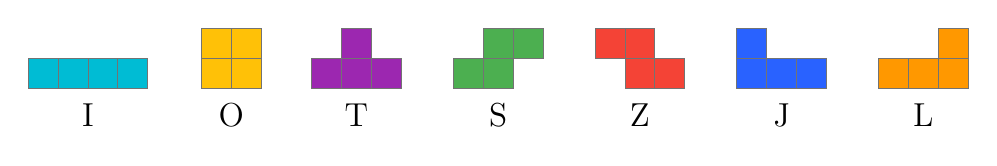
\begin{tikzpicture}[scale=1]
  \def\csz{0.38}
  \begin{scope}[shift={(0,0)}]    \tetro{0/0,1/0,2/0,3/0}{tI}{\csz}   \node at (0.76,-0.35) {I}; \end{scope}
  \begin{scope}[shift={(2.2,0)}]  \tetro{0/0,1/0,0/1,1/1}{tO}{\csz}   \node at (0.38,-0.35) {O}; \end{scope}
  \begin{scope}[shift={(3.6,0)}]  \tetro{0/0,1/0,2/0,1/1}{tT}{\csz}   \node at (0.57,-0.35) {T}; \end{scope}
  \begin{scope}[shift={(5.4,0)}]  \tetro{0/0,1/0,1/1,2/1}{tS}{\csz}   \node at (0.57,-0.35) {S}; \end{scope}
  \begin{scope}[shift={(7.2,0)}]  \tetro{0/1,1/1,1/0,2/0}{tZ}{\csz}   \node at (0.57,-0.35) {Z}; \end{scope}
  \begin{scope}[shift={(9.0,0)}]  \tetro{0/0,1/0,2/0,0/1}{tJ}{\csz}   \node at (0.57,-0.35) {J}; \end{scope}
  \begin{scope}[shift={(10.8,0)}] \tetro{0/0,1/0,2/0,2/1}{tL}{\csz}   \node at (0.57,-0.35) {L}; \end{scope}
\end{tikzpicture}
\caption{Bảy loại khối gạch trong Tetris (hình minh họa do nhóm vẽ)}
\end{figure}

\textbf{Kinh nghiệm chơi:} Khối I (thanh dài) rất hợp để xóa nhiều hàng cùng lúc; khối O (hình vuông) gọn gàng, không cần xoay; khối S và Z dễ để lại khe hở nếu đặt vội; khối T linh hoạt; còn J và L tiện để lấp các góc.

\subsection{Cách chơi dành cho người dùng cuối}
\textbf{Mục tiêu:} Xếp các khối rơi xuống sao cho lấp kín các hàng ngang để ghi điểm, và cố chơi được lâu nhất có thể trước khi đống gạch chất cao tới đỉnh.

\textbf{Luật chơi cơ bản:}
\begin{enumerate}
  \item Khung chơi là một hình chữ nhật có tường hai bên và đáy.
  \item Mỗi lần có một khối mới xuất hiện ở phía trên và tự rơi xuống từng nấc.
  \item Bạn có thể dịch khối sang trái, sang phải, cho rơi nhanh hơn hoặc xoay khối trước khi nó chạm đáy.
  \item Khối dừng lại khi chạm đáy hoặc chạm một khối khác, rồi trở thành một phần của ``đống gạch''.
  \item Hàng ngang nào không còn ô trống sẽ bị xóa, các hàng phía trên rơi xuống thế chỗ và bạn được cộng điểm.
  \item Ngay sau đó một khối mới xuất hiện và vòng chơi tiếp tục.
\end{enumerate}

\textbf{Xóa hàng như thế nào?} Hình~\ref{fig:xoahang} minh họa một tình huống thường gặp: hai hàng dưới cùng chỉ còn thiếu đúng một ô ở cùng một cột. Khi thả khối I thẳng đứng vào khe đó, hai hàng cùng đầy và bị xóa một lúc. Xóa nhiều hàng cùng lúc luôn được nhiều điểm hơn xóa từng hàng.

\begin{figure}[H]
\centering
\begin{tikzpicture}[scale=1]
  \def\csz{0.42}
  % ---- Trước: bảng 8 cột x 6 hàng
  \begin{scope}
    \foreach \r in {0,1}{\foreach \col in {0,1,2,3,4,6,7}{
      \fill[gray!55,draw=black!55,line width=0.3pt] (\col*\csz,\r*\csz) rectangle ++(\csz,\csz);}}
    \tetro{5/2,5/3,5/4,5/5}{tI}{\csz}
    \draw[line width=1pt] (0,6*\csz) -- (0,0) -- (8*\csz,0) -- (8*\csz,6*\csz);
    \node[align=center,font=\small] at (4*\csz,-0.7) {Khối I đang rơi\\vào khe trống};
  \end{scope}
  \draw[-{Stealth[length=3mm]},line width=1pt] (4.2,1.1) -- (5.4,1.1);
  % ---- Sau
  \begin{scope}[shift={(6,0)}]
    \tetro{5/0,5/1}{tI}{\csz}
    \draw[line width=1pt] (0,6*\csz) -- (0,0) -- (8*\csz,0) -- (8*\csz,6*\csz);
    \node[align=center,font=\small] at (4*\csz,-0.7) {Hai hàng đầy\\bị xóa cùng lúc};
  \end{scope}
\end{tikzpicture}
\caption{Ví dụ xóa hai hàng cùng lúc (hình minh họa do nhóm vẽ)}
\label{fig:xoahang}
\end{figure}

\textbf{Điều khiển:} Phiên bản của nhóm dự kiến bám theo bộ phím trong mã khởi tạo của giảng viên và bổ sung thêm phím xoay, tạm dừng.

\begin{table}[H]
\centering

\begin{tabularx}{\linewidth}{|c|X|X|}
\hline
\textbf{Phím} & \multicolumn{1}{c|}{\textbf{Chức năng}} & \multicolumn{1}{c|}{\textbf{Ghi chú}} \\ \hline
\texttt{a} & Dịch khối sang trái & Có sẵn trong mã khởi tạo \\ \hline
\texttt{d} & Dịch khối sang phải & Có sẵn trong mã khởi tạo \\ \hline
\texttt{x} & Cho khối rơi nhanh xuống & Có sẵn trong mã khởi tạo \\ \hline
\texttt{w} & Xoay khối 90$^\circ$ & Nhóm sẽ bổ sung \\ \hline
\texttt{p} & Tạm dừng / tiếp tục & Nhóm sẽ bổ sung \\ \hline
\texttt{q} & Thoát game & Có sẵn trong mã khởi tạo \\ \hline
\end{tabularx}
\vspace{8pt}
\caption{Phím điều khiển của game}
\label{tab:dieukhien}
\end{table}

\textbf{Khi nào game kết thúc?} Khi khối mới không còn chỗ để xuất hiện ở phía trên (đống gạch đã chạm tới đỉnh), game báo ``Game Over''. Người chơi có thể chọn chơi lại để thử phá kỷ lục của chính mình.

\textbf{Mẹo cho người mới:}
\begin{itemize}
  \item Giữ đống gạch thấp và phẳng, tránh để lại những ``giếng'' sâu mà chỉ khối I mới lấp được.
  \item Đừng vội cho rơi nhanh khi chưa chắc vị trí; sai một nước có thể mất cả hàng.
  \item Nhìn trước khối kế tiếp (nếu game có hiển thị) để lên kế hoạch nước đi.
  \item Ưu tiên lấp các ô trống bị che bên dưới trước khi xếp tiếp lên trên.
\end{itemize}

\subsection{Các chức năng chính}\label{sec:chucnang}
Từ cách chơi ở trên, nhóm chia chức năng của game làm hai nhóm: \emph{cơ bản} (bám theo khung mã và video của giảng viên) và \emph{mở rộng} (nhóm tự bổ sung).

\begin{table}[H]
\centering

\begin{tabularx}{\linewidth}{|c|p{2.8cm}|X|>{\centering\arraybackslash}p{2.7cm}|}
\hline
\textbf{Nhóm} & \multicolumn{1}{c|}{\textbf{Chức năng}} & \multicolumn{1}{c|}{\textbf{Mô tả}} & \textbf{Trong mã khởi tạo} \\ \hline
Cơ bản & Bảng chơi & Khung chơi có tường hai bên và đáy, lưu bằng mảng hai chiều ký tự & \texttt{board}, \texttt{initBoard} \\ \hline
Cơ bản & Khối gạch & Mỗi khối là ma trận 4$\times$4; ô trống là dấu cách & \texttt{blocks} \\ \hline
Cơ bản & Di chuyển & Dịch trái, phải và cho rơi nhanh xuống bằng phím & \texttt{a}, \texttt{d}, \texttt{x} \\ \hline
Cơ bản & Rơi tự động & Khối tự rơi từng nấc theo thời gian & vòng lặp \texttt{main} \\ \hline
Cơ bản & Kiểm tra va chạm & Không cho khối đi xuyên tường, đáy hoặc khối khác & \texttt{canMove} \\ \hline
Cơ bản & Cố định khối & Khối chạm đáy hoặc khối khác thì dính vào bảng & \texttt{block2Board} \\ \hline
Cơ bản & Xóa hàng đầy & Hàng không còn ô trống bị xóa, các hàng trên rơi xuống & \texttt{removeLine} \\ \hline
Cơ bản & Sinh khối mới & Sau khi khối cố định, tạo khối ngẫu nhiên ở phía trên & \texttt{rand} \\ \hline
Cơ bản & Hiển thị console & Vẽ lại toàn bộ bảng sau mỗi bước & \texttt{draw} \\ \hline
Mở rộng & Đủ 7 loại khối & Chuẩn hóa mảng \texttt{blocks}: mỗi loại I, O, T, S, Z, J, L đúng một khối, đúng như Tetris gốc & --- \\ \hline
Mở rộng & Xoay khối & Xoay 90$^\circ$; không cho xoay khi vướng tường hoặc khối khác & --- \\ \hline
Mở rộng & Game over & Báo thua khi khối mới không còn chỗ xuất hiện & --- \\ \hline
Mở rộng & Điểm, level, tốc độ & Tính điểm theo số hàng xóa, tăng level và tăng dần tốc độ rơi & --- \\ \hline
Mở rộng & Giao diện đẹp & Màu theo loại khối, khung thông tin, hiển thị khối kế tiếp & --- \\ \hline
Mở rộng & Menu, tạm dừng, chơi lại & Màn hình bắt đầu, phím tạm dừng, hỏi chơi lại sau khi thua & --- \\ \hline
\end{tabularx}
\vspace{8pt}
\caption{Các chức năng chính của game}
\label{tab:chucnang}
\end{table}
\textbf{Định hướng thiết kế:} Game được viết bằng C++ và chạy trên console. Toàn bộ bảng chơi là một mảng ký tự hai chiều, các khối là ma trận ký tự 4$\times$4, và logic của game xoay quanh bốn việc: vẽ bảng, đặt/xóa khối trên bảng, kiểm tra va chạm và xóa hàng đầy. Đây cũng là cách chia chức năng để các thành viên làm song song trên các nhánh Git riêng mà ít đụng nhau.

% =====================================================================
%  PHÂN CÔNG VÀ KẾT QUẢ THỰC HIỆN CỦA TỪNG THÀNH VIÊN
%  Đối chiếu: nhiệm vụ trong hợp đồng nhóm <-> mã nguồn src/ <-> lịch sử Git
%  (rà soát trực tiếp từ repository tại commit cf0d48f)
% =====================================================================

\label{sec:contributions}

Phần này đối chiếu nhiệm vụ đã cam kết trong hợp đồng nhóm (Mục~1, Bảng~\ref{tab:phancong})
với những gì thực sự tồn tại trong mã nguồn tại thời điểm báo cáo. Mỗi đầu việc của
thành viên được dẫn chiếu đến tệp, hàm tương ứng trong thư mục \texttt{src/} và bằng
chứng từ lịch sử Git (nhánh, Pull Request).


% ============================================================
%  TÀI LIỆU THAM KHẢO
% ============================================================
% ============================================================
%  TÀI LIỆU THAM KHẢO
% ============================================================
\clearpage
\titleformat{name=\section,numberless}[block]
  {\raggedright\fontsize{14pt}{21pt}\selectfont\bfseries\color{black}}
  {}{0pt}{\MakeUppercase}
\phantomsection
\addcontentsline{toc}{section}{TÀI LIỆU THAM KHẢO}

\begin{thebibliography}{9}
\setlength{\itemsep}{6pt}

\bibitem{gomagic}
GoMagic, ``Play Tetris Online,'' \textit{GoMagic} (phiên bản Tetris thông dụng được giảng viên minh họa). [Trực tuyến]. Địa chỉ: \url{https://gomagic.org/play-tetris/}. 

\bibitem{video}
Giảng viên môn SS004.R11, ``Video hướng dẫn cách lập trình game Tetris,'' \textit{YouTube}. [Trực tuyến]. Địa chỉ: \url{https://youtu.be/vcXaTVjdlJ0}.

\bibitem{wiki}
Wikipedia, ``Tetris,'' \textit{Wikipedia, The Free Encyclopedia}. [Trực tuyến]. Địa chỉ: \url{https://en.wikipedia.org/wiki/Tetris}. 

\end{thebibliography}
\end{document}
